\documentclass{beamer}

\usepackage[utf8]{inputenc}
\usepackage{fancybox}
\usepackage{environ}
\usepackage{tikz}

\beamertemplatenavigationsymbolsempty

\title{1.3 Differential Equations \\ as Mathematical Models}

\subtitle{a lesson for MATH F302 Differential Equations}

\author{Ed Bueler, Dept.~of Mathematics and Statistics, UAF}

\date{\tiny \today}


\usetheme{Pittsburgh}


\begin{document}

\setbeamertemplate{itemize item}{$\bullet$}
\setbeamertemplate{itemize subitem}{$\circ$}


\begin{frame}
\titlepage

\centerline{\tiny for textbook: \, D. Zill, \emph{A First Course in Differential Equations with Modeling Applications}, 11th ed.}
%\color{green!40!blue}
\end{frame}


\begin{frame}{DEs as models}

\begin{itemize}
\item I have already described differential equations models
    \begin{itemize}
    \item made a big deal of it in previous slides!
    \end{itemize}
\item for section \S 1.3 my plan is:
    \begin{itemize}
    \item I will work-through several exercises in these slides, and
    \item \emph{you} will actually read the examples in the section
    \end{itemize}
\end{itemize}
\end{frame}

\begin{frame}{exercise 2 in \S 1.3}

\scriptsize
\begin{quotation}
\noindent \textbf{2}.  The population model given in (1) fails to take death into consideration: the growth rate equals the birth rate.  In another model of a changing population of a community it is assumed that the rate at which the population changes is a \emph{net} rate---that is, the difference between the rate of births and the rate of deaths in the community.  Determine a model for the population $P(t)$ if both the birth rate and the death rate are proportional to the population present at time $t>0$.
\end{quotation}

\small
\vspace{-3mm}

\begin{itemize}
\item the population model in (1) is simply that the rate of change of population is proportional to the population: $\frac{dP}{dt} = k P$
\item this exercise asks for ``another model'' where ``both the birth rate and death rate are proportional'' to $P(t)$
    \begin{itemize}
    \item $P(t) =$ ``the population present at time $t>0$''
    \end{itemize}
\item in the new model we want $\frac{dP}{dt}$ to be the \emph{net} rate
\item the net rate is ``the difference between the rate of births and the rate of deaths''
\end{itemize}
\end{frame}


\begin{frame}{exercise 2 cont.}

\begin{itemize}
\item the rate at which the population changes is net rate:
    $$\frac{dP}{dt} = (\text{rate of births}) - (\text{rate of deaths})$$
\item both the birth rate and death rate are proportional to $P(t)$:
\begin{align*}
    (\text{rate of births}) &= k_b P \\
    (\text{rate of deaths}) &= k_d P
\end{align*}
where $k_b,k_d$ are two new \emph{positive} constants
\end{itemize}
\end{frame}


\begin{frame}{exercise 2 cont.~cont.}

\begin{itemize}
\item the new model combines the stuff on last slide:
    $$\frac{dP}{dt} = k_b P - k_d P = (k_b-k_d) P$$
\item thus new model is really the old model (1):
    $$\frac{dP}{dt} = k P \quad \text{ where } k = k_b-k_d$$

\bigskip
\item \emph{conclusion}.  by thinking this through we see that (1) \emph{already allowed} births and deaths, with $k=k_b-k_d$

\bigskip
\item \alert{please go back and actually \emph{read} the ``Population Dynamics'' example on page 23}
\end{itemize}
\end{frame}


\begin{frame}{exercise 5 in \S 1.3}

\scriptsize
\begin{quotation}
\noindent \textbf{5}.  A cup of coffee cools according to Newton's law of cooling (3).  Use data from the graph of temperature $T(t)$ [below] to estimate the constants $T_m$, $T_0$, and $k$ in a model of the form of a first order initial-value problem: $dT/dt = k(T-T_0)$, $T(0)=T_0$.
\end{quotation}

\begin{itemize}
\item X
\end{itemize}

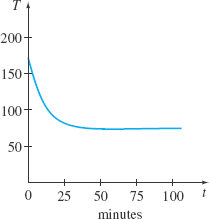
\includegraphics[width=0.4\textwidth]{exercise-5-1-3}
\end{frame}


\begin{frame}{exercise 21 in \S 1.3}

\begin{itemize}
\item X
\end{itemize}

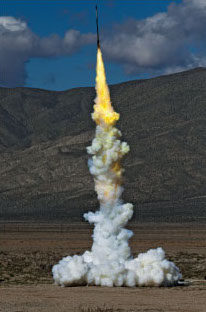
\includegraphics[width=0.25\textwidth]{exercise-21-1-3}
\end{frame}


\begin{frame}{X}

\begin{itemize}
\item X
\end{itemize}
\end{frame}


\begin{frame}{X}

\begin{itemize}
\item X
\end{itemize}
\end{frame}


\begin{frame}{X}

\begin{itemize}
\item X
\end{itemize}
\end{frame}


\begin{frame}{X}

\begin{itemize}
\item X
\end{itemize}
\end{frame}


\begin{frame}{X}

\begin{itemize}
\item X
\end{itemize}
\end{frame}


\begin{frame}{X}

\begin{itemize}
\item X
\end{itemize}
\end{frame}


\begin{frame}{X}

\begin{itemize}
\item X
\end{itemize}
\end{frame}


\begin{frame}{expectations}

to learn this material, just watching this video is \emph{not} enough; also
\begin{itemize}
\item \emph{read} section 1.3 in the textbook
\item \emph{do} the WebAssign exercises for section 1.3
\item see the other ``found online'' videos at the bottom of the week 2 page:
\end{itemize}

\centerline{\href{https://bueler.github.io/math302/week2.html}{\tt \color{cyan} bueler.github.io/math302/week2.html}}
\end{frame}

\end{document}

